\section{Use Cases}

Udviklingen af løsningen er sket på baggrund af de forudgående analyser, samt diskussioner og overvejelser omkring mulige vinkler hvorfra problemet kan gribes an. Som en del af processen blev der udarbejdet use cases.

Det gøres for at udpensle sandsynlige arbejdsmønstre for den tiltænkte løsning, og for at normalisere ideer om interaktion med systemet.

Der er mange forskellige tilgange til use cases, men de tager udgangspunkt i det samme princip. I denne rapport er use cases lavet efter kapitel 17 i \enquote{Agile Principles, Patterns, and Practices in C\#} \cite{martin2006agile}. Denne bog er valgt fordi den har en simpel tilgang til use cases. Her følger en beskrivelse af use cases som præsenteret i \cite{martin2006agile}.

En use case er i simpleste forstand en følge af trin, der bliver udført mellem en person, kaldet aktøren, og et system. Traditionelt er en use case skrevet meget udførlig, men \cite{martin2006agile} mener at use cases handler om, at skrive det primære forløb af interaktionen. Ved at gøre det simpelt, sikres det, at der ikke bliver brugt tid på at diskutere punkter, der ikke er essentielle.

Trin i use cases tager udgangspunkt i et problemfrit forløb. Dertil kan skrives et alternativt forløb til sandsynlige afvigelser fra den problemfrie brug.

\subsection*{Use Case Diagram}

For at visualisere et systems use case, opsættes et use case diagram. Dette diagram visualiserer de aktuelle aktøre samt systemet og dets funktioner. I diagrammet er systemet repræsenteret som en aflang rektangel, og use cases repræsenteres af de ovale cirkler. Alt inden for rektanglet er systemet som er udviklet. Uden for systemet ses aktørerne samt hvilke use cases de kan interagere med, som er repræsenteret af linjerne. En af fordelene ved at lave dette diagram, er at der skabes et overblik, samt en bedre forståelse af hvilke aktørere der interagere med hvilke use cases. Diagrammet kaldes ofte for et \enquote{System Boundary Diagram} fordi det effektivt visualisere et systems grænser. På \cref{fig:usecase} ses et use case diagram for LOBOP.

\begin{figure}
  \centering
    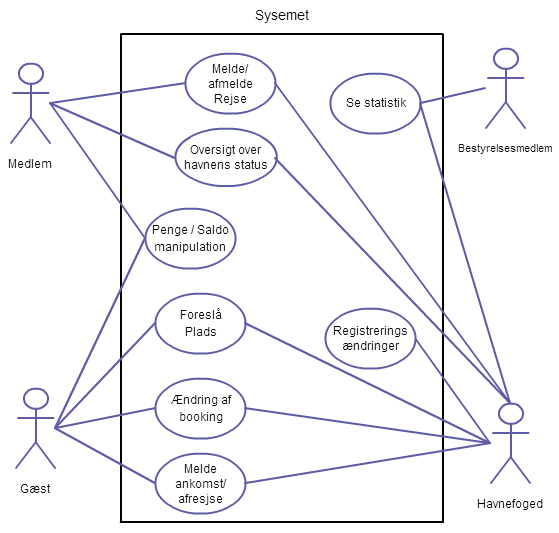
\includegraphics[width=\textwidth]{use_case_diagram.png}
  \caption{LOBOP System boundary diagram}
  \label{fig:usecase}
\end{figure}